\documentclass[conference]{IEEEtran}
\usepackage{graphicx}

\hyphenation{op-tical net-works semi-conduc-tor}

\begin{document}

\title{Exploring Binary Classification in Supervised Learning: Comparative Analysis of Red Wine Quality and Mushroom Edibility Using ML Algorithms}

\author{\IEEEauthorblockN{Randy Agüero Bermúdez}
\IEEEauthorblockA{\textit{Escuela de Ciencias de la Computación e Informática} \\
\textit{Universidad de Costa Rica}\\
San José, Costa Rica \\
randy.aguero@ucr.ac.cr}
\and
\IEEEauthorblockN{Sara Espinoza Hernández.}
\IEEEauthorblockA{\textit{Escuela de Ciencias de la Computación e Informática} \\
\textit{Universidad de Costa Rica}\\
San José, Costa Rica \\
sara.espinoza@ucr.ac.cr}
\and
\IEEEauthorblockN{Andrés Quesada González}
\IEEEauthorblockA{\textit{Escuela de Ciencias de la Computación e Informática} \\
\textit{Universidad de Costa Rica}\\
San José, Costa Rica \\
andres.quesadagonzalez@ucr.ac.cr}
\and
\IEEEauthorblockN{Queene Zavala Morales.}
\IEEEauthorblockA{\textit{Escuela de Ciencias de la Computación e Informática} \\
\textit{Universidad de Costa Rica}\\
San José, Costa Rica \\
queene.zavala@ucr.ac.cr}
}

\maketitle

\begin{abstract}
  The present study explores the application of supervised learning approaches to binary classification problems, taking into consideration two different datasets: Red Wine Quality and the Mushroom Dataset. The effort involves data preprocessing, feature selection, and the application of four different machine learning algorithms, namely Logistic Regression, Decision Trees, k-Nearest Neighbors (kNN), and Neural Networks. These algorithms' performance evaluations are done via hyperparameter optimization and iteration of experiments with the help of various metrics such as accuracy, precision, recall, and ROC-AUC. The results will contain the fundamental relations of the tradeoffs that exist between model complexity and generalization, with computational efficiency regarding the chosen datasets. To be more specific, in the Red Wine dataset, wines are labeled as high or low according to their physicochemical properties, while the Mushroom dataset involves classifying mushrooms into edible and toxic groups. The findings emphasize feature selection, dataset characteristics, and algorithm selection for achieving optimum classification performance. over-fitting and under-fitting, as well as the reproducibility of the results across experiments, are discussed in this paper, which comprehensively evaluates various methodologies related to supervised learning.
\end{abstract}

\begin{IEEEkeywords}
  supervised learning, binary classification, wine, mushrooms, machine learning algorithms, logistic regression, decision trees, k-nearest neighbors, neural networks, model evaluation metrics, machine learning, ai.
  \end{IEEEkeywords}

\section{Introduction}
Texto inicial.*

\subsection{Background}
Introduce el problema de clasificación binaria y su importancia en Machine Learning.

\subsection{Objective}
Explica los objetivos específicos del proyecto, como la comparación de algoritmos y el análisis de datasets.

\section{Methodology}

\subsection{Datasets}
The project utilized two datasets to explore binary classification problems:

1. Red Wine Quality Dataset
The Wine Quality dataset includes 11 features of the physicochemical properties of red wine samples, taken from the UCI Machine Learning Repository (Cortez et al., 2009). These wines vary in alcohol content, acidity, and levels of sulfur dioxide, among other characteristics. The variable of interest, in this case, is wine quality, rated on a continuous scale between 3 and 8. For the purpose of this project, the ratings have been split into two clear-cut classes: "low quality" (3–5) and "high quality" (6–8), making a binary classification problem. This above-mentioned dataset contains more than 1,500 entries, which makes it very suitable for testing various classifiers. 

2. Mushroom Dataset
The Mushroom dataset, by Prisha Sawhney 2024, is used to classify mushrooms as either edible or poisonous.
Some of the features in this dataset include cap shape, odour, and spore print color, to name a few. These collectively provide great insight into the mushrooms. The target variable is binary, where it tells whether the mushroom is edible or toxic. This dataset contains thousands of rows of data, which will be a great benchmark to examine the generalization capability of machine learning models in a different domain. 

This two datasets were chosen for the diversity of their attributes, a unique binary classification structure, and adequate size to enable efficient experimentation and analysis of different machine learning algorithms.

\subsection{Data Preprocessing}

\subsection{Feature selection}
Feature selection was purposely done before training to make the models more efficient and, if possible, improve their effectiveness. By only focusing on the most relevant features, the models have managed to elude useless information, therefore improving interpretability and at the same time keeping good predictive accuracy. It was an informed process based on the unique characteristics of each dataset, making sure that it included only those variables that contributed substantially to classification. In cases where features were believed to be redundant, all features were preserved to avoid losing potentially important information. This systematic approach made sure that the feature selection process supported the experiments without introducing inappropriate constraints.

\subsection{Machine Learning Algorithms}
\subsubsection{Logistic Regression}
\subsubsection{Decision Trees}
Decision Trees are among the most widely used machine learning algorithms for classification tasks due to their interpretability, simplicity, and ease in capturing non-linear relationships in data. The algorithm partitions the data into subsets based on the decision rules derived from the input features and builds a tree-like structure. They are quite effective but susceptible to over-fitting, which might be eased by techniques such as either limiting tree depth or pruning. This work used Decision Trees to determine their effectiveness on classification and also to explore the importance of some features in the data sets.

\subsubsection{k-Nearest Neighbors}
\subsubsection{Neural Networks}

\subsection{Hyperparameter Optimization}

\subsection{Experimental Setup}
\subsection{Model Evaluation Metrics}


\section{Results and Discussion}
\subsection{Red Wine Quality Dataset}
\subsubsection{Logistic Regression}
\subsubsection{Decision Trees} The Decision Tree model applied to the Wine Quality dataset underlines effectively, for wine quality prediction, the most influential features. In this respect, feature importance stands for the impurity reduction of the created splits by the Decision Tree for a given feature. It provides a quantitative view about the importance of each physicochemical characteristic in the classification of wine quality.

\begin{figure}[h] 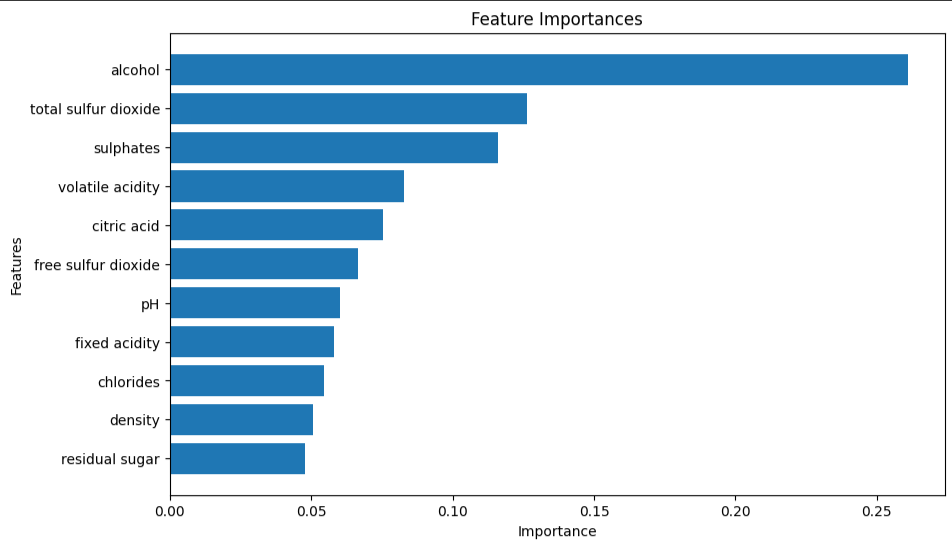
\includegraphics[width=\columnwidth]{plots/dt_wine_feature_importance.png} \caption{Feature Importance for Decision Tree Model on Wine Quality Dataset} \label{fig:dt_feature_importance_wine} \end{figure}

Therefore, according to Figure \ref{fig:dt_feature_importance_wine} the feature importance analysis for the Decision Tree model on Wine Quality Dataset shows that alcohol is the most important feature, hence a major divisor for the model to distinguish between different grades of quality. Some other important features include total sulfur dioxide, sulfates, and volatile acidity, which most in feature importance contribute to the model's classification mechanism.

\textbf{Optimization and Hyperparameter Selection}:
The structure of the Decision Tree was optimized using a systematic GridSearch approach in order to find the set of the best performing hyperparameters. The selected hyperparameters were the following:

\textbf{Criterion:} Entropy
\textbf{Maximum Depth:} 10
\textbf{Minimum Samples per Leaf:} 32
\textbf{Minimum Samples to Split:} 92

Hence, hyperparameter tuning had to be carried out with the goal of minimum overfitting for maximum generality. Optimization was accordingly extended to 5-fold cross-validation with the intention of making the evaluation performance of the model robust and repeatable. Feature pruning is adopted by choosing some impactful features like alcohol, total sulfur dioxide, and volatile acidity, based on their Gini importance according to impurity reduction. This yields a simpler interpretable model with no loss in predictive accuracy.

\begin{table}[h]
\centering
\caption{Performance Metrics for Decision Tree Model on Wine Quality Dataset}
\label{tab:dt_wine}
\begin{tabular}{|l|c|c|}
\hline
\textbf{Metric} & \textbf{Train Mean} & \textbf{Test Mean} \\
\hline
Accuracy & 0.771 & 0.738 \\
\hline
Precision & 0.789 & 0.765 \\
\hline
Recall & 0.780 & 0.737 \\
\hline
AUC & 0.854 & 0.801 \\
\hline
\end{tabular}
\end{table}

\begin{figure}[h] \centering 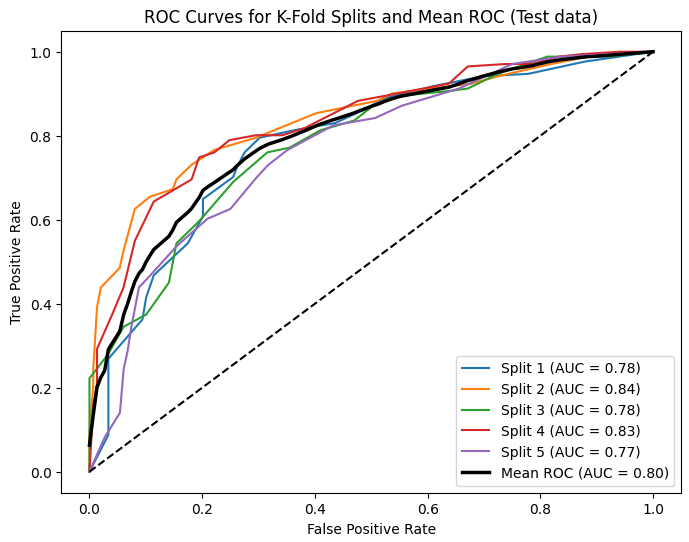
\includegraphics[width=\columnwidth]{plots/dt_wine_ROC_curves.png} \caption{ROC Curves for Decision Tree Model on Wine Quality Dataset} \label{fig:dt_roc_wine} \end{figure}

Table \ref{tab:dt_wine} demonstrates that the model achieved a testing accuracy of 73.8\%, complemented by a mean AUC of 0.801, indicating robust overall performance. This conclusion is further supported by Figure \ref{fig:dt_roc_wine}, which highlights the ROC curves across cross-validation folds. These curves consistently exhibit high discriminatory power, with a mean AUC of 0.80, aligning with the earlier result of 76.5\% precision. The Decision Tree's ability to effectively balance true positives and false positives is reinforced by the graphical representation, where the ROC curves display minimal variation across folds, confirming consistent performance around the mean.

Moreover, the "mean cross-validation accuracy" of the dataset was 73.04\%, which speaks to the stability in predictive performance across all splits. That would align with the ability of the Decision Tree to generalize well on unseen data with a reliance on features like alcohol and sulfur dioxide driving predictive outcomes. Also, the Decision Tree model has higher accuracy on the training set compared to the test set, which hints at overfitting. The overfitting isn't high enough to confirm that the model is too reliant on the training data, which is a good indication. This was the common problem with Decision Trees, and there were some reduction methods, like pruning or just limiting the depth of the tree.

However, despite these strengths, the decision tree is limited in its tendency toward underfitting complex relationships due to focusing on one single feature at every split. For example, "volatile acidity" and "citric acid," although important, may have interactions that univariate splits would fail to notice. This limits the indication that while Decision Trees are well-mannered in terms of interpretability, they lack the required subtlety for datasets entailing complex feature interdependencies. Which can explain the model's performance, that is good but not excellent.

\subsubsection{k-Nearest Neighbors}
\subsubsection{Neural Networks}

\subsection{Mushroom Dataset}
\subsubsection{Logistic Regression}
\subsubsection{Decision Trees}
\subsubsection{k-Nearest Neighbors}
\subsubsection{Neural Networks}

\subsection{General Discussion}

\section{Conclusion}
The conclusion goes here.

\nocite{*}
\def\BibTeX{BibTeX}
\bibliographystyle{IEEEtran}
\bibliography{IEEEabrv,./refs}

\end{document}
